This section introduces the first kind arithmetic expression space ($\mathfrak{E}_1$), providing a geometric framework for analyzing arithmetic expressions. The space is constructed on the upper half-plane with a hyperbolic metric: $ds^2 = \frac{1}{y^2} (dx^2 + dy^2)$, where the assignment function $a = - \frac{x}{y}$ satisfies the flow equation and serves as an eigenfunction of the Laplacian with eigenvalue 2.

Two equivalent examples of $\mathfrak{E}_1$ are presented: the upper half-plane model and a horocycle-based coordinate system, connected through Möbius transformation. The section explores geometric propagation mechanisms, showing how the assignment value propagates like expanding concentric circles in hyperbolic space. It examines grid structures in $\mathfrak{E}_1$, revealing dual grids reflecting the geometric structure of the Baumslag-Solitar group, and demonstrates how arithmetic torsion corresponds precisely to hyperbolic areas enclosed between evaluation paths. The section concludes by introducing tube structures, which extend $\mathfrak{E}_1$ to parameterized families, enabling analysis of how expressions evolve across parameter variations.

\subsection{Foundational exemplars}\label{subsec:motivexamples}

We present two analytically equivalent examples that belong to the class of spaces designated as the first kind arithmetic expression space $\mathfrak{E}_1$.

\subsubsection{Example 1: Upper Half Plane Model}

Consider the upper half plane ${\mathcal{H}: (x, y) \ | \ y > 0}$ equipped with the following inner product and metric tensor:

$$
\mathbf{a} \cdot \mathbf{b} = \begin{bmatrix} a_x & a_y \end{bmatrix} \begin{bmatrix} \frac{1}{y^2} & 0 \\ 0 & \frac{1}{y^2} \end{bmatrix} \begin{bmatrix} b_x \\ b_y \end{bmatrix}
$$

$$
ds^2 = \frac{1}{y^2} (dx^2 + dy^2)
$$

On this manifold, we define an assignment field $a$ as follows:

\begin{equation}\label{eq:exmp1}
a = - \frac{x}{y}
\end{equation}

\begin{theorem}\label{thm:exmp1}
The assignment $a$ defined by formula \eqref{eq:exmp1} satisfies the flow equation \eqref{eq:flow}.
\end{theorem}

\begin{proof}
We initiate with the differential of the assignment:
$$
da = d\left(-\frac{x}{y}\right) = \frac{xdy - ydx}{y^2} = -\frac{dx + ady}{y}
$$

The differential of arc length is given by:
$$
ds = \frac{\sqrt{dx^2 + dy^2}}{y}
$$

Therefore:
$$
\frac{da}{ds} = - \frac{dx + ady}{y} \cdot \frac{y}{\sqrt{dx^2 + dy^2}} = - \frac{dx + ady}{\sqrt{dx^2 + dy^2}}
$$

In the local coordinate system determined by $(-1, 0)$ and $(0, -1)$ under the right-hand rule, we have:
$$
\cos \theta = \frac{-dx}{\sqrt{dx^2 + dy^2}} \quad \text{and} \quad \sin \theta = \frac{-dy}{\sqrt{dx^2 + dy^2}}
$$

Substituting these values:
$$
\frac{da}{ds} = \cos \theta + a \sin \theta
$$

This precisely corresponds to the flow equation \eqref{eq:flow} with $\mu=1$ and $\lambda=1$.
\end{proof}

We can verify that $a$ constitutes an eigenfunction of the Laplacian operator:
$$
\Delta a = - y^2 \left(\frac{\partial^2 a}{\partial x^2} + \frac{\partial^2 a}{\partial y^2}\right) = y^2 \left(\frac{\partial}{\partial y} \left(\frac{\partial}{\partial y} \frac{x}{y}\right)\right) = 2a
$$

\subsubsection{Example 2: Horocycle-Based Coordinate System}

For our second exemplar, we introduce a horocycle-based coordinate system for hyperbolic surfaces. This global coordinate system comprises two orthogonal families of curves: horocycles sharing the same ideal point, and geodesics perpendicular to these horocycles.

\begin{figure}[ht]
\centering
\resizebox{0.5\textwidth}{!}{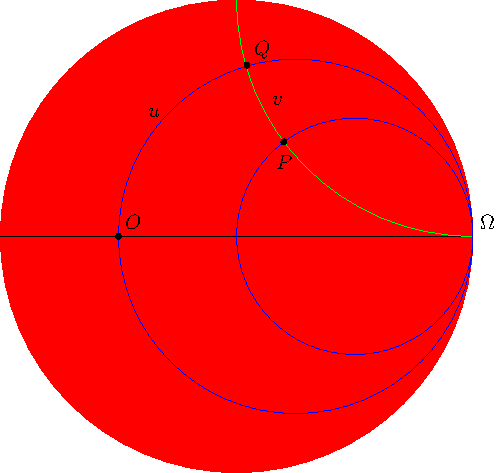
\includegraphics{images/11-horocyclebased}}
\caption{A horocycle-based coordinate system on the Poincaré disc. Blue curves represent horocycles tangent at ideal point $\Omega$, green lines depict perpendicular geodesics.}\label{fig:horocyclecoord}
\end{figure}

On the Poincaré disc $\mathcal{P}$, the coordinates of a point $P$ are denoted by $(u,v)$, where:
\begin{itemize}
\item $u$ represents the signed length of $OQ$
\item $v$ represents the signed length of $QP$
\item The sign conventions adhere to the right-hand rule and orientation relative to the ideal point $\Omega$
\end{itemize}

We equip this coordinate system with the inner product:
$$
\mathbf{a} \cdot \mathbf{b} = \begin{bmatrix} a_u & a_v \end{bmatrix} \begin{bmatrix} e^{-2v} & 0 \\ 0 & 1 \end{bmatrix} \begin{bmatrix} b_u \\ b_v \end{bmatrix}
$$

And the corresponding metric tensor:
$$
ds^2 = e^{-2v} du^2 + dv^2
$$

The Laplacian operator in this coordinate system is expressed as:
$$
\Delta = e^{2v} \frac{\partial^2}{{\partial u}^2} + \frac{\partial^2}{{\partial v}^2} - \frac{\partial}{\partial v}
$$

In this coordinate framework, we define an assignment:

\begin{equation}\label{eq:exmp2}
a = u e^{-v}
\end{equation}

\begin{theorem}\label{thm:exmp2}
The assignment $a$ defined by formula \eqref{eq:exmp2} satisfies the flow equation \eqref{eq:flow}.
\end{theorem}

\begin{proof}
We establish this result by demonstrating that examples 1 and 2 are equivalent through a Möbius transformation. Consider the complex representation of the upper half plane:
$$
z = x + yi
$$

The Möbius transformation mapping the upper half plane to the Poincaré disc is given by:
$$
z \mapsto \frac{z-i}{z+i}
$$

\begin{figure}[ht]
\centering
\resizebox{0.8\textwidth}{!}{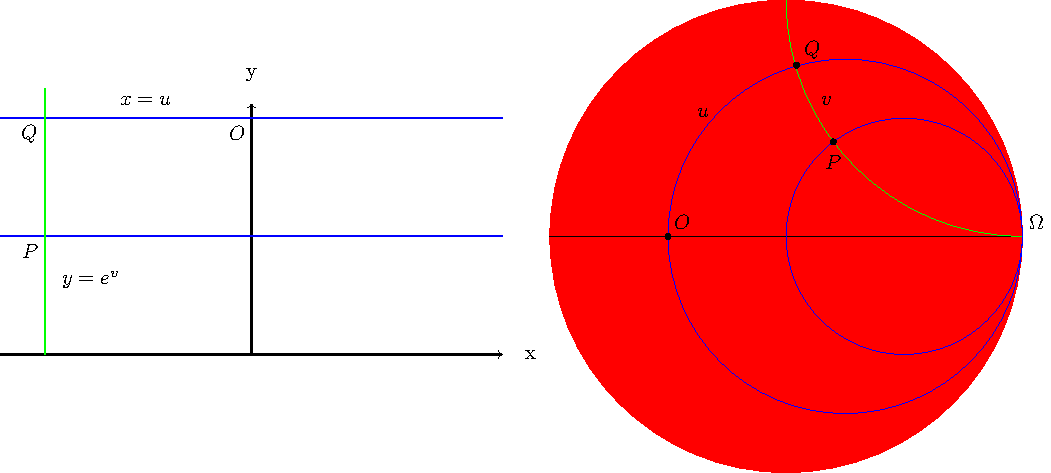
\includegraphics{images/12-proofbymapping}}
\caption{Mapping between the upper half plane and Poincaré disc models}\label{fig:mapping}
\end{figure}

This conformal transformation maps horizontal lines in $\mathcal{H}$ to horocycles sharing the ideal point $\Omega = 1$ in $\mathcal{P}$, and vertical geodesics in $\mathcal{H}$ to perpendicular geodesics in $\mathcal{P}$.

Expressed in the target coordinate system, this transformation yields:
$$
\begin{cases}
x = u\\
y = e^v \\
\end{cases}
$$

Substituting into the assignment from Example 1:
$$
a = -\frac{x}{y} = -\frac{u}{e^v} = -u e^{-v}
$$

Since the Möbius transformation is conformal and preserves the flow equation, and accounting for the orientation change, we obtain $a = u e^{-v}$ satisfying the flow equation.
\end{proof}

As in Example 1, we can verify that $a$ constitutes an eigenfunction of the Laplacian:
$$
\Delta a = e^{2v} \frac{\partial^2(u e^{-v})}{{\partial u}^2} + \frac{\partial^2(u e^{-v})}{{\partial v}^2} - \frac{\partial(u e^{-v})}{\partial v} = 2a
$$

These two examples, emerging from the same geometric foundation but expressed in different coordinate systems, demonstrate the fundamental properties of the first kind arithmetic expression space.

\subsection{Theoretical framework of $\mathfrak{E}_1$ space}\label{subsec:generalframework}

Building upon the foundational exemplars, we now establish a comprehensive theoretical framework for the first kind arithmetic expression space $\mathfrak{E}_1$. 

Consider the upper half plane $\mathcal{B}$:
$$
\{\mathcal{B}: (x, y) | y > 0 \}
$$

equipped with an inner product and metric tensor parameterized by constants $\mu$ and $\lambda$:

$$
\mathbf{a} \cdot \mathbf{b} = \begin{bmatrix} a_x & a_y \end{bmatrix} \begin{bmatrix} \frac{1}{\mu^2 y^2} & 0 \\ 0 & \frac{1}{\lambda^2 y^2} \end{bmatrix} \begin{bmatrix} b_x \\ b_y \end{bmatrix}
$$

$$
ds^2 = \frac{1}{y^2}\left(\frac{dx^2}{\mu^2} + \frac{dy^2}{\lambda^2}\right)
$$

The assignment function in this generalized framework maintains the form:

\begin{equation}\label{eq:genassignment}
a = - \frac{x}{y}
\end{equation}

This defines the first kind arithmetic expression space $\mathfrak{E}_1$, characterized by the following theorem:

\begin{theorem}\label{thm:generalE1}
The assignment $a$ given by \eqref{eq:genassignment} satisfies the flow equation \eqref{eq:flow} with parameters $\mu$ and $\lambda$, independent of the specific values of these generators.
\end{theorem}

\begin{proof}
The differential of the assignment is given by:
$$
da = d\left(-\frac{x}{y}\right) = \frac{xdy - ydx}{y^2} = -\frac{dx + a dy}{y}
$$

The differential of arc length is expressed as:
$$
ds = \frac{1}{y}\sqrt{\frac{dx^2}{\mu^2} + \frac{dy^2}{\lambda^2}}
$$

Therefore:
$$
\frac{da}{ds} = - \frac{dx + a dy}{y} \cdot \frac{y}{\sqrt{\frac{dx^2}{\mu^2} + \frac{dy^2}{\lambda^2}}} = -\frac{dx + a dy}{\sqrt{\frac{dx^2}{\mu^2} + \frac{dy^2}{\lambda^2}}}
$$

In the local coordinate system determined by $(-1, 0)$ and $(0, -1)$ according to the right-hand rule:

$$
\cos \theta = \frac{-\frac{dx}{\mu}}{\sqrt{\frac{dx^2}{\mu^2} + \frac{dy^2}{\lambda^2}}} \quad \text{and} \quad \sin \theta = \frac{-\frac{dy}{\lambda}}{\sqrt{\frac{dx^2}{\mu^2} + \frac{dy^2}{\lambda^2}}}
$$

Substituting these values:
$$
\frac{da}{ds} = \mu \cos \theta + a \lambda \sin \theta
$$

This precisely corresponds to the flow equation \eqref{eq:flow} with the given parameters $\mu$ and $\lambda$.
\end{proof}

The $\mathfrak{E}_1$ space is distinguished by its intrinsic connection to hyperbolic geometry and the property that the assignment function $a = -x/y$ constitutes an eigenfunction of the Laplacian operator with eigenvalue 2. This space provides a natural geometric framework for analyzing arithmetic expressions, particularly those involving addition and multiplication operations.

\subsection{Geometric propagation mechanisms}\label{subsec:geompropagation}

The flow equation \eqref{eq:flow} in the $\mathfrak{E}_1$ space, $da/ds = \mu \cos \theta + a \lambda \sin \theta$, provides a dynamic interpretation of arithmetic expression evaluation as a propagation process. This perspective extends the propagation method discussed in Section \ref{subsec:propagation-method}.

We can visualize this process using the concept of wavefronts. Considering the locus where the assignment $a=0$ (the y-axis, $x=0$) as the initial source or baseline, the "information" or "value" propagates outwards into the upper half-plane $\mathcal{H}$. The flow equation governs how the assignment value $a$ changes as this propagation occurs.

Points with the same assignment value form equipotential lines, or contours, defined by $a = -x/y = a_0$ (constant). In the $(x,y)$ coordinate chart of $\mathcal{H}$, these contours are rays emanating from the origin, described by the equation $x = -a_0 y$.

A key insight arises when observing how these equipotential lines behave as the propagation proceeds. Propagation, fundamentally occurring along directions related to the gradient of $a$ (which are orthogonal to the contours), leads to an increase in the magnitude $|a|$ as points move further from the initial $a=0$ line.

Now, consider the orientation of the contour ray $x = -a_0 y$. Its slope in the $(x,y)$ plane is $dy/dx = -1/a_0$.
\begin{itemize}
    \item When $|a_0|$ is very small (i.e., close to the initial $a=0$ state on the y-axis), the slope $-1/a_0$ is very large in magnitude, meaning the ray is nearly vertical, aligned closely with the y-axis.
    \item As the wavefront propagates outwards, the magnitude $|a_0|$ increases. Consequently, the magnitude of the slope $|-1/a_0|$ decreases, approaching zero as $|a_0| \to \infty$. This means the ray becomes increasingly horizontal, aligning more closely with the x-axis.
\end{itemize}
Therefore, the geometric propagation driven by the flow equation manifests as a dynamic \textbf{sweeping or change in orientation of the equipotential rays} $a=a_0$. As the magnitude $|a|$ increases due to propagation away from the zero line, the corresponding ray appears to \textbf{rotate} from a near-vertical orientation (along the y-axis for $a=0$) towards a near-horizontal orientation (along the positive x-axis if $a \to -\infty$, or the negative x-axis if $a \to +\infty$).

This increase in magnitude $|a|$ with the propagation distance $s$ along the gradient is quantified by the relationship $|a| = (\mu/\lambda) \sinh(\lambda s)$ (derived from \eqref{eq:gradevo5} for propagation from $a_0=0$), confirming that further propagation indeed leads to larger $|a|$ values and thus more horizontally oriented contour lines.

This dynamic picture of equipotential rays sweeping from vertical towards horizontal alignment provides a core geometric interpretation of the propagation mechanism inherent in the flow equation within the $\mathfrak{E}_1$ space.

\subsection{Grid structures}\label{subsec:grids}

A significant geometric characteristic of the first kind arithmetic expression space is the presence of two distinct yet interrelated grid structures, each encoding addition and multiplication operations in different ways. These dual grids reflect the geometric structure of the Baumslag–Solitar group, whose Cayley graph exhibits an anisotropic, hierarchical lattice with a natural correspondence to mixed additive-multiplicative expressions.

Both grid structures are constructed within the upper half-plane model. The first grid is rectilinear, consisting of horizontal lines encoding addition operations and vertical lines encoding multiplication operations. Specifically, this grid is constructed through iterative applications of these two operations to generate a lattice in the $(x,y)$ coordinates. Each horizontal displacement from $(x,y)$ to $(x+1,y)$ represents an addition, and each vertical displacement from $(x,y)$ to $(x,2y)$ represents a multiplication by 2. The grid vertices correspond to values of expressions constructed from repeated applications of addition and multiplication operations, typically originating from a rational base point, often designated as 1.

\begin{figure}[ht]
\centering
\resizebox{0.8\textwidth}{!}{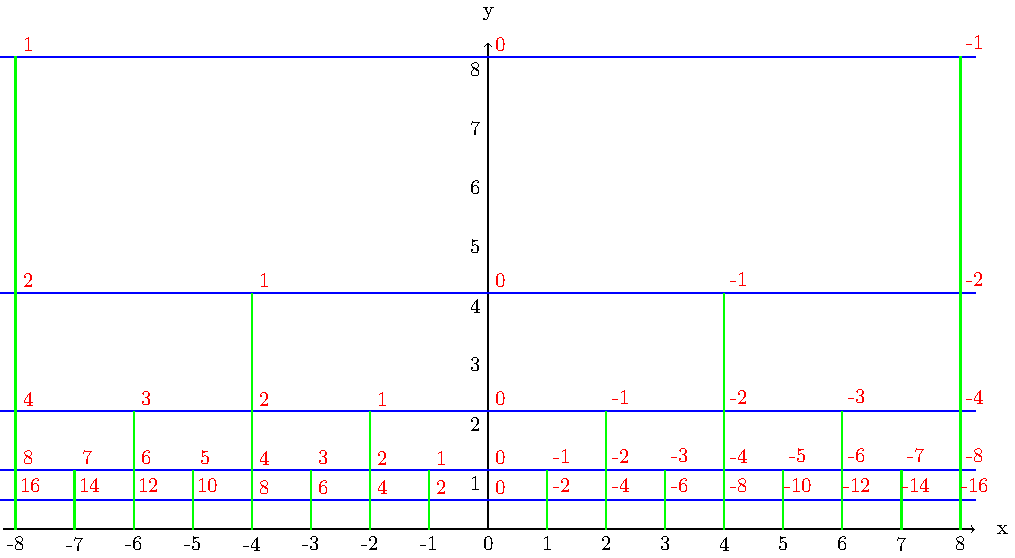
\includegraphics{images/01-grid-example-1}}
\caption{Rectilinear grid structure in the first kind arithmetic expression space $\mathfrak{E}_1$}\label{fig:grid1}
\end{figure}

Notably, in this first grid, the scalar field $a$ remains invariant under variations of the metric parameters $\mu$ and $\lambda$. That is, while the geometric properties of the space (lengths and angles) vary with these parameters, the locus where $a=0$—specifically, the vertical line $x=0$—remains structurally invariant and unaffected by changes in $\mu$ and $\lambda$.

The second grid emerges through a conformal transformation, specifically the Möbius transformation acting within the upper half-plane. This transformation maps horizontal lines to semicircles centered on the real axis and vertical rays to orthogonal semicircles. Under this transformation, the roles of addition and multiplication are effectively interchanged. The addition-multiplication structure of the first grid transforms into a new system of curved geodesics: the images of addition steps now follow curved trajectories around the origin, while the multiplicative steps exhibit contraction and inversion properties.

\begin{figure}[ht]
\centering
\resizebox{0.8\textwidth}{!}{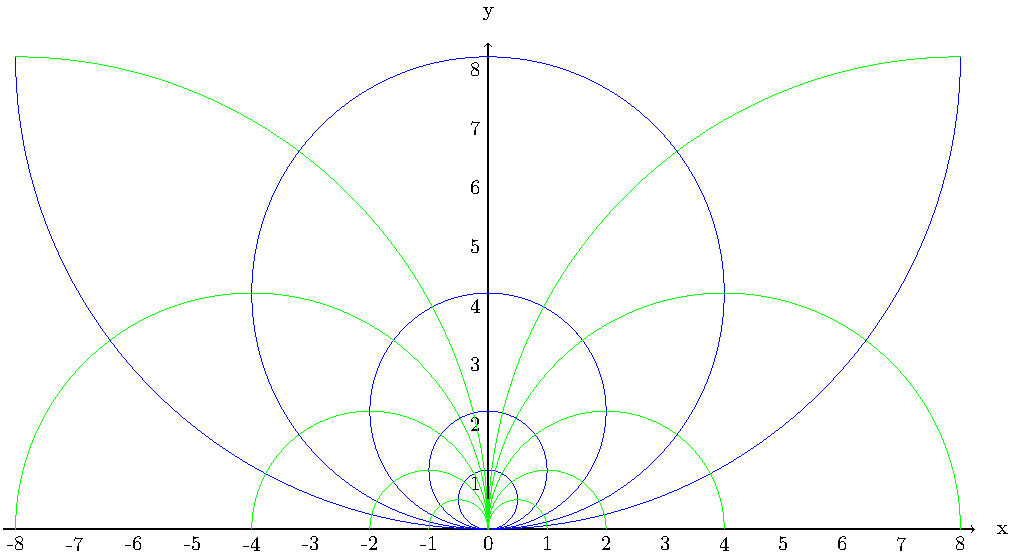
\includegraphics{images/18-grid-example-2}}
\caption{Transformed grid structure in the first kind arithmetic expression space $\mathfrak{E}_1$}\label{fig:grid2}
\end{figure}

Although the visual structure of the second grid exhibits greater complexity, it retains a profound arithmetic coherence. The grid vertices continue to correspond to expressions generated through repeated applications of addition and multiplication operations, albeit composed under the transformed geometry. This grid demonstrates enhanced flexibility: under the conformal transformation, the images of zero lines such as $x=0$ are no longer fixed but deform into dynamic arcs. Consequently, the second grid accommodates a richer family of zero structures, allowing for the possibility of curved, branching, or nested nodal sets that vary with $\mu$, $\lambda$, or the choice of conformal framing.

Each of these grid structures can be interpreted as a geometric realization of a Cayley graph:

\begin{itemize}
\item The rectilinear grid corresponds to the Cayley graph of the Baumslag–Solitar group $BS(1,2)$, where multiplication by 2 followed by addition by 1 follows the relation $b^{-1}ab = a^2$.
\item The transformed (dual) grid corresponds to the Cayley graph of the dual Baumslag–Solitar group, where the roles of addition and multiplication are inverted.
\end{itemize}

Thus, the two grid systems exhibit duality not only in geometric terms but also in group-theoretic structure. The Möbius transformation, acting within the upper half-plane, connects these dual groups by exchanging generators and inverting flow directions, reflecting an intrinsic duality in the geometric composition of arithmetic operations.

The coexistence of these dual grid structures—one linear, one curved—linked via conformal symmetry, suggests a profound underlying symmetry in the geometry of arithmetic expressions. This duality reflects how different evaluation paths or expression embeddings can be interpreted as projections from a common, more complex geometric source. Understanding this symmetry may provide a pathway to expressing arithmetic relations via modular or automorphic structures, particularly in the context of recursive expressions and iterative identities, where Baumslag–Solitar-like behavior naturally emerges.

We conjecture that this grid duality corresponds to a deeper expression-theoretic equivalence, and that the Möbius transformation connecting them manifests an underlying arithmetic symmetry in expression geometry.

\subsection{Torsion under scale transformation}\label{subsec:gridsandtorsion}

The addition-multiplication grid introduced in Section~\ref{subsec:meshgrid} has a natural embedding in the arithmetic expression space $\mathfrak{E}_1$. This grid consists of two orthogonal families of curves:

\begin{enumerate}
    \item \textbf{Addition curves} (blue lines): horizontal geodesics along which $y$ remains constant, representing iterated additions.
    \item \textbf{Multiplication curves} (green lines): vertical or logarithmically scaled geodesics where the ratio $x/y$ remains constant, representing multiplicative transformations.
\end{enumerate}

This grid structure facilitates the geometric analysis of \emph{arithmetic torsion}—a quantity arising from the non-commutativity of certain additive and multiplicative expression sequences. Specifically, torsion quantifies the discrepancy between two seemingly equivalent but differently ordered expressions.

\begin{figure}[ht]
    \centering
    \resizebox{0.8\textwidth}{!}{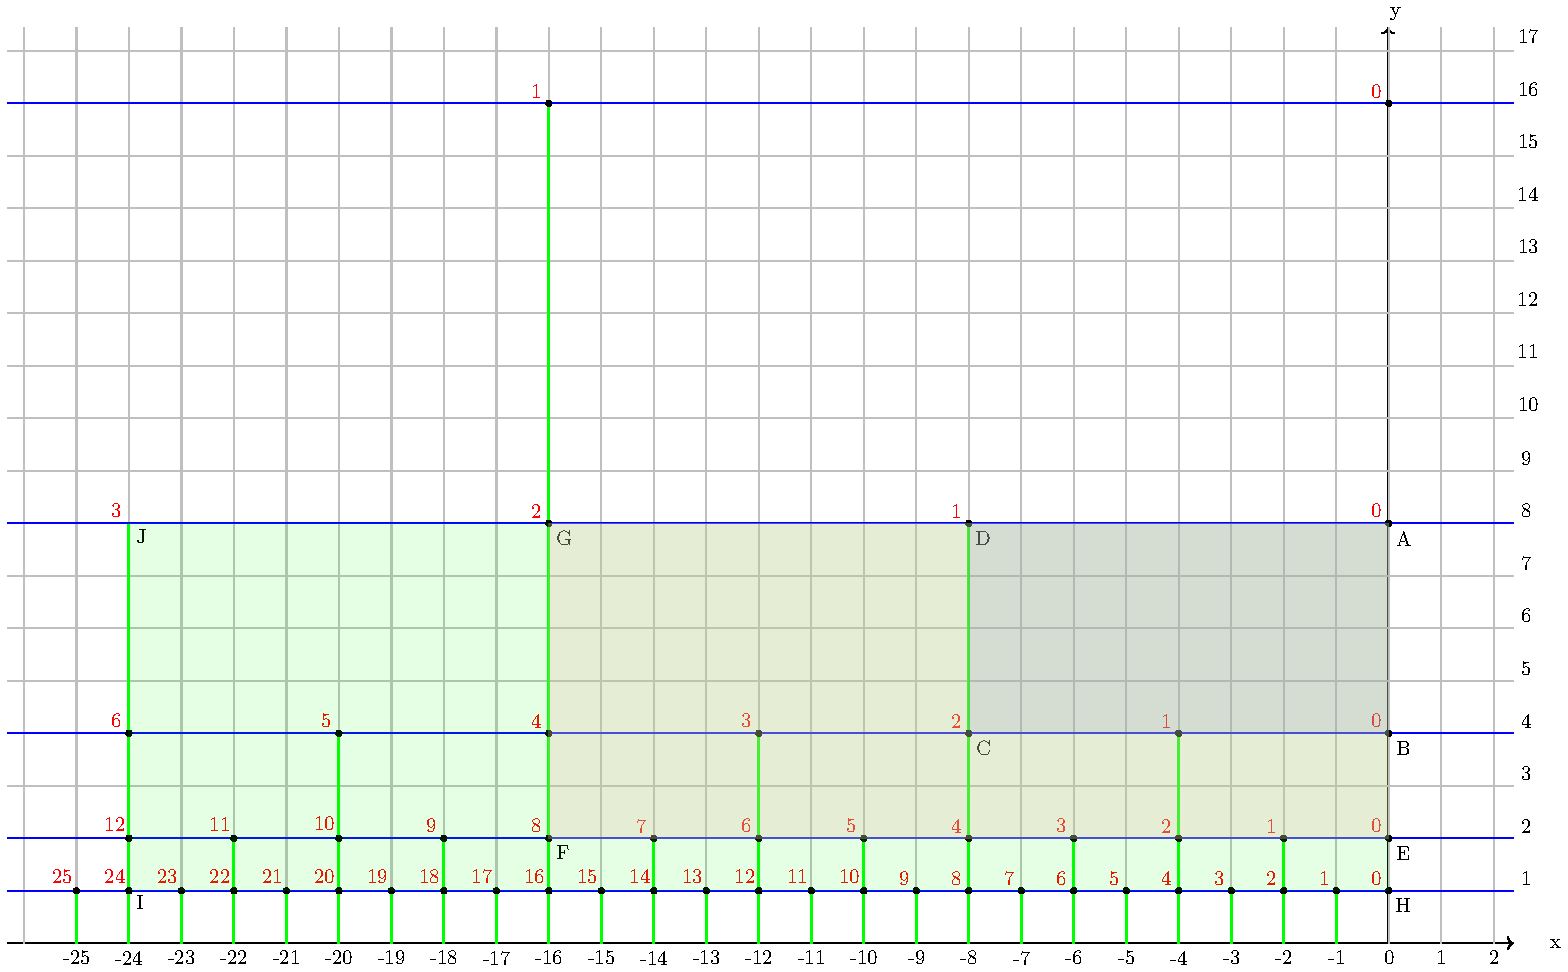
\includegraphics{images/17-area-formula}}
    \caption{Illustration of the correspondence between hyperbolic area and arithmetic torsion}\label{fig:area-formula}
\end{figure}

Figure~\ref{fig:area-formula} illustrates the relationship between the area enclosed by expression paths in the grid and the resulting torsion. Consider the following expression identity comparisons:

\begin{itemize}
    \item One-step case:
    \begin{equation}
        x \times 2 + 1 - (x + 1) \times 2 = -1
    \end{equation}

    \item Two-step case:
    \begin{equation}
        x \times 4 + 2 - (x + 2) \times 4 = -6
    \end{equation}

    \item Three-step case:
    \begin{equation}
        x \times 8 + 3 - (x + 3) \times 8 = -21
    \end{equation}
\end{itemize}

These differences correspond precisely to the hyperbolic areas enclosed between alternative evaluation paths within these specific grid examples:

\begin{itemize}
    \item The region $ABCD$ encompasses 1 unit cell.
    \item The region $AEFG$ encompasses 6 unit cells.
    \item The region $AHIJ$ encompasses 21 unit cells.
\end{itemize}
These examples compellingly suggest that arithmetic torsion accumulates in proportion to the area enclosed by the grid paths, indicating a potential connection between algebraic non-commutativity and geometric surface area.

Further supporting this connection, we established a differential formulation:
\begin{equation}
    d\tau = \mu \lambda\, du\, dv \label{eq:area_formula}
\end{equation}
where $d\tau$ represents the infinitesimal arithmetic torsion, and $du\, dv$ denotes the area element in the $(u, v)$ coordinate system adapted to the grid. This equation provides the precise microscopic law linking infinitesimal torsion to the infinitesimal area element.

However, while we possess both macroscopic observations suggesting a torsion-area relationship (from the scaled grid examples) and the exact microscopic differential law \eqref{eq:area_formula}, the explicit integral theorem rigorously bridging these scales is currently underdeveloped. Formulating how the microscopic torsion density $d\tau$ integrates over a finite region to yield the total accumulated torsion—potentially involving boundary terms in analogy with Stokes' theorem, or relating the total torsion to curvature and topology similarly to the Gauss-Bonnet theorem—remains a key objective for future work.

The analogy with curvature in differential geometry therefore becomes particularly pertinent: just as Gaussian curvature encodes deviation from flatness, arithmetic torsion quantifies deviation from commutativity in arithmetic flow. In this sense, torsion constitutes a measure of the operational significance of evaluation order.

The $\mathfrak{E}_1$ space thus provides a mathematical framework where algebraic non-commutativity manifests as measurable geometric distortion—establishing a novel interpretation of arithmetic structure as a form of discrete curvature. This opens avenues for investigating further geometric invariants such as torsion density, torsion-induced flow bifurcation, and \textbf{realizing} a Gauss–Bonnet-type integral identity for arithmetic surfaces.

\subsection{Tube structure}\label{sec:tubestructure}

In preceding sections, we introduced the first kind arithmetic expression space $\mathfrak{E}_1$ as a geometric realization of arithmetic flow under \textbf{fixed} generator parameters $\mu$ and $\lambda$. However, more complex structures emerge when we consider the entire family of spaces indexed by the parameter $\lambda$ (or potentially both $\mu$ and $\lambda$) and analyze how expression behavior evolves across this family. This naturally leads to the concept of a \emph{tube structure}.

\subsubsection{From Slices to Parameterized Families}\label{subsec:tube_slices}

Each individual $\mathfrak{E}_1$ space, denoted $\mathfrak{E}_1^{(\lambda)}$, can be conceptualized as a single \emph{slice} or \emph{fiber} (in the sense of fiber bundles) within the family of expression spaces indexed by the parameter $\lambda$. Within each slice, the evaluation of arithmetic expressions is realized through traversal along (geodesic) paths, the result is governed by the scalar field $a$, and the flow is determined by the metric tensor corresponding to that slice.

Consider a fixed algebraic structure—for instance, an alternating path (with a fixed internal multiplier) corresponding to a polynomial $P(x)$—and examine how its evaluation result $P(e^\lambda)$ evolves as the tube structure parameter $\lambda$ varies. For each value of $\lambda$, the evaluation $P(e^\lambda)$ corresponds to a point (or more accurately, the assignment value $a$ at that point) within the $\lambda$-slice $\mathfrak{E}_1^{(\lambda)}$. As $\lambda$ varies continuously, these points trace out a continuous trajectory through the family of spaces. We refer to such a trajectory generated by $P$ as a \emph{section} or a \emph{$\lambda$-trajectory}. The collection of all slices corresponding to the allowed $\lambda$ values, along with these structures upon them, together form a new, higher-dimensional entity: the tube structure.

\subsubsection{Tube Structure as Total Space}\label{subsec:tube_total_space}

We define a \textbf{tube structure $\mathcal{T}$} as the \emph{total space} formed by the family of $\mathfrak{E}_1$ spaces indexed by a continuous parameter $\lambda$ (typically $\lambda > 0$), which can be formally written as the disjoint union:
\begin{equation}
\mathcal{T} = \bigsqcup_{\lambda > 0} \mathfrak{E}_1^{(\lambda)}
\end{equation}
This total space needs to be endowed with an appropriate topology (and possibly a differential or fiber bundle structure) to support coherent analysis along the $\lambda$-direction.

In this structure:
\begin{itemize}
    \item The \emph{base space} is the parameter domain $\Lambda$ for $\lambda$ (e.g., $\mathbb{R}^+$).
    \item The \emph{fiber} over each point $\lambda$ in the base space is the geometric expression space $\mathfrak{E}_1^{(\lambda)}$.
    \item Fixed algebraic expression structures (especially those corresponding to polynomials $P(x)$, via the evaluation $P(e^\lambda)$) trace \emph{canonical sections} or $\lambda$-trajectories through $\mathcal{T}$. These sections connect the fibers for different $\lambda$.
\end{itemize}

\subsubsection{Zero Loci and Nodal Evolution}\label{subsec:tube_zeros}

A primary motivation for studying tube structures is to investigate how \emph{zero loci}—the sets of points where an expression evaluates to zero ($a=0$)—evolve with the parameter $\lambda$.

\begin{itemize}
    \item \textbf{In the Tube Structure $\mathcal{T}_1$ based on $\mathfrak{E}_1$}: For the $\mathfrak{E}_1$ space ($a=-x/y$) that we have discussed in detail, the zero locus within \textbf{each slice} $\mathfrak{E}_1^{(\lambda)}$ is always the \textbf{same simple} line: the y-axis ($x=0$). Consequently, in the tube structure $\mathcal{T}_1 = \bigsqcup \mathfrak{E}_1^{(\lambda)}$, the overall zero locus is the trivial hyperplane $x=0$.

    \item \textbf{Outlook for Non-Trivial Spaces}: However, as our research suggests, the simplicity of the zero locus in $\mathfrak{E}_1$ might limit its capacity to explain more complex phenomena (like those observed in knot theory examples). Therefore, there is strong motivation to seek and construct \textbf{"non-trivial" arithmetic expression spaces $\mathfrak{E}_{NT}$}, where a single slice $\mathfrak{E}_{NT}^{(\lambda)}$ might possess \textbf{multiple or morphologically more complex zero lines}. In the tube structures $\mathcal{T}_{NT}$ built from such non-trivial spaces, the zero locus itself could evolve with $\lambda$, potentially exhibiting various interesting phenomena, such as:
    \begin{itemize}
        \item \textbf{Bifurcation}: New zero lines might emerge or merge with existing ones as $\lambda$ varies.
        \item \textbf{Branching}: The zero locus of certain expressions might exhibit multi-valued behavior along the $\lambda$-direction.
        \item \textbf{Topology change}: The overall zero surface might develop handles (genus), singularities, or undergo other changes in its topological structure.
    \end{itemize}
\end{itemize}
The analysis of such complex zero loci and their evolution (potentially within $\mathcal{T}_{NT}$) constitutes a core direction for studying expression dynamics, particularly when considering families of expressions or differential equations involving $\lambda$.

\subsubsection{Investigative Approaches and Outlook}\label{subsec:tube_outlook}

The formalism of tube structures opens up multiple avenues for research in arithmetic expression geometry:

\begin{itemize}
    \item Examining the global properties of zero surfaces (in the general case where they might be non-trivial), such as their genus, regions of curvature concentration, and dependence on the parameter $\lambda$.
    \item Studying the geometric properties of sections $\gamma_P$ corresponding to polynomials $P(e^\lambda)$ within the tube structure, and investigating whether imposing geometric continuity conditions leads to algebraic rigidity.
    \item Exploring the possibility of establishing flow equations across the $\lambda$-family, perhaps defining a notion of \emph{connection} or \emph{parallel transport} between different $\lambda$-slices.
    \item Defining \emph{moduli spaces} of expression geometries as structured fiber bundles over parameter spaces.
\end{itemize}

Ultimately, tube structures provide a mathematical framework wherein the dynamics of arithmetic expressions can be analyzed analogously to field theory. In this analogy, expressions (or their underlying algebraic structures) act as structured sections, while quantities like arithmetic torsion, curvature, and zero loci serve as local or global invariants.